%% LaTeX2e class for student theses
%% sections/content.tex
%% 
%% Karlsruhe Institute of Technology
%% Institute for Program Structures and Data Organization
%% Chair for Software Design and Quality (SDQ)
%%
%% Dr.-Ing. Erik Burger
%% burger@kit.edu
%%
%% Version 1.3.3, 2018-04-17

\chapter{Visualization Methods}
\label{ch:Visualization}
In this chapter, we first introduce the correlation matrix in \autoref{sec:Visualization:CorrelationMatrix} and then introduce three useful interactive visualization methods \autoref{sec:Visualization:Heatmap} Heatmap, \autoref{sec:Visualization:BarGraph} Bar Graph and \autoref{sec:Visualization:ForceDirectedGraph} Force-Directed-Graph, and give examples of each visualization method using the same data set in \autoref{sec:Visualization:mtcars}.\\

\section{Correlation Matrix}
\label{sec:Visualization:CorrelationMatrix}
The most familiar measure of dependence between two quantities is the Pearson product-moment correlation coefficient\cite{correlation}, known as "Pearson's correlation coefficient". It is obtained by dividing the covariance of the two variables by the product of their standard deviations. The population correlation coefficient $\rho _{X,Y}$ between two random variables $X$ and $Y$ and standard deviations $\sigma _{X}$ and $\sigma_Y$ is defined as
\begin{equation}
\rho _{X,Y}=\operatorname {corr} (X,Y)={\operatorname {cov} (X,Y) \over \sigma _{X}\sigma _{Y}}
\end{equation}
where $\operatorname {cov}$ means covariance, and $\operatorname {corr}$ is a widely used alternative notation for the correlation coefficient. The Pearson correlation is defined only if both of the standard deviations are finite and non-zero.\\
The standard tool of correlation analysis is the computation of a correlation matrix
\begin{equation}
\rho = \begin{bmatrix}
	\rho_{1,1} & \dots & \rho_{1,n} \\ 
	\dots & \dots & \dots \\ 
	\rho_{n,1} & \dots & \rho_{n,n}
\end{bmatrix}
n \in \mathcal{N}^*
\end{equation}
for n variables. The correlation matrix is used to investigate the dependence between multiple variables at the same time. In fact, we are only interested in the lower half of the matrix because of its symmetry and invariant diagonal line.\\

\section{Data Set Mtcars}
\label{sec:Visualization:mtcars}
Data Set Mtcars represents Auto MPG Data Set, which can be found in UCI Machine Learning Repository by url: https://archive.ics.uci.edu/ml/datasets/auto+mpg. It is a data frame with 32 observations on 11 variables. This data set can be seen as a standard data set widely-used in the field of data analysis. \autoref{sec:Visualization:Heatmap}, \autoref{sec:Visualization:BarGraph} and \autoref{sec:Visualization:ForceDirectedGraph} all use this data set to visualize.

\section{Heatmap}
\label{sec:Visualization:Heatmap}
A common visualization is the heatmap\cite{heatmap}, which is originated in 2D displays of the values in a data matrix. The \autoref{fig:Heatmap} is a heatmap of a correlation matrix, in which the variables with strong correlation (high values) are printed in light colour and those with low correlation are in dark colour.\\

\section{Bar Graph}
\label{sec:Visualization:BarGraph}
A bar graph\cite{bar} presents categorical data with rectangular bars with heights or lengths proportional to the values that they represent. We use vertical bar graph in our developed interface. In a vertical bar graph, the x-Axis shows the specific categories being compared, and the y-Axis represents a measured value, which is the correlation value in our situation. Bar graphs provide a visual presentation of categorical data, which are usually qualitative. \autoref{fig:Bar Graph} is a bar graph, using the same data set in \autoref{fig:Heatmap}.\\

\section{Force-Directed-Graph}
\label{sec:Visualization:ForceDirectedGraph}
Force-Directed-Graph\cite{force} assigns forces among the set of edges and the set of nodes of a graph drawing. The purpose of it is to position the nodes of a graph in two-dimensional or three-dimensional space so that all the edges are of more or less equal length and there are as few crossing edges as possible. In such a simulation, the forces are applied to the nodes, pulling them closer together or pushing them further apart. This can be used to simulate the relationship of different attributes throughout the time. \autoref{fig:Force-Directed-Graph} is the example of Force-Directed-Graph, which also uses Data Set Mtcars.\\
\begin{figure}[h]
	\centering
	\begin{subfigure}[b]{0.32\textwidth}
		\centering
		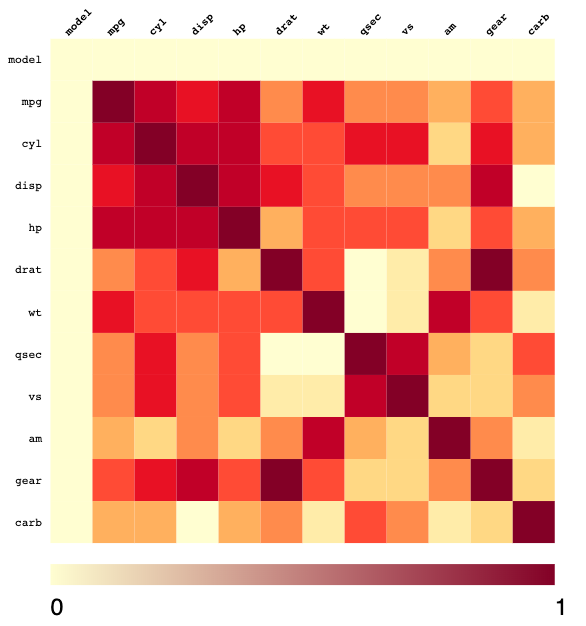
\includegraphics[width=\textwidth]{pictures/correlationMatrix}
		\caption{Heatmap as the visualization method}
		\label{fig:Heatmap}
	\end{subfigure}
	\hfill
	\begin{subfigure}[b]{0.32\textwidth}
		\centering
		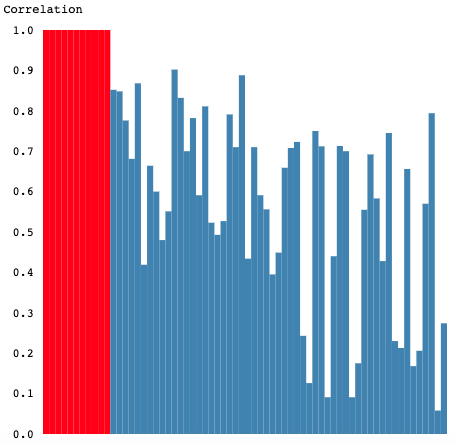
\includegraphics[width=\textwidth]{pictures/bg}
		\caption{Bar Graph as the visualization method}
		\label{fig:Bar Graph}
	\end{subfigure}
	\hfill
	\begin{subfigure}[b]{0.32\textwidth}
		\centering
		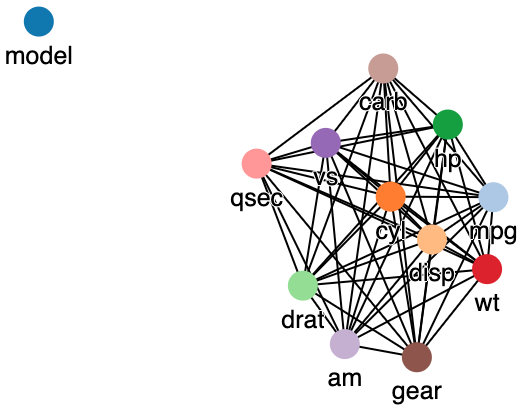
\includegraphics[width=\textwidth]{pictures/fdg}
		\caption{Force-Directed-Graph as the visualization method}
		\label{fig:Force-Directed-Graph}
	\end{subfigure}
	\caption{Three visualization methods of the Data Set Mtcars}
	\label{fig:vis}
\end{figure}
